\section{Introduction}

Economic participants drive markets towards equilibrium. This process, however, is contrained by the
technical properties of the currency used. This paper describes these technical properties and shows
how, by correctly isolating and controlling previously coupled components, effective control of
currency can be achieved that is highly likely to lead to sustained, stable, aggregate economic
equilibrium with full-employment. Around 1741 David Hume \cite{hume1741} observed that real economic
conditions were affected by increases in money supply, which he noted was contrary to the notion
that increases in the price as unit of measurement should be independent of the real factors,

\begin{quotation}
\fontsize{8pt}{8pt}

``If we consider any one kingdom by itself, it is evident, that the greater or less plenty of money is
    of no consequence; since the prices of commodities are always proportioned to the plenty of
    money, and a crown in Harry VII.’s time served the same purpose as a pound does at present ...
    It is indeed evident, that money is nothing but the representation of labour and commodities,
    and serves only as a method of rating or estimating them. Where coin is in greater plenty; as a
    greater quantity of it is required to represent the same quantity of goods; it can have no
    effect, either good or bad, taking a nation within itself; any more than it would make an
    alteration on a merchant’s books, if, instead of the Arabian method of notation, which requires
    few characters, he should make use of the Roman, which requires a great many ... \textbf{But
    notwithstanding this conclusion}, which must be allowed just, it is certain, that, since the
    discovery of the mines in America, industry has encreased in all the nations of Europe, except
    in the possessors of those mines; and this may justly be ascribed, amongst other reasons, to the
    encrease of gold and silver.  Accordingly we find, that, in every kingdom, into which money
    begins to flow in greater abundance than formerly, every thing takes a new face: labour and
    industry gain life; the merchant becomes more enterprising, the manufacturer more diligent and
    skilful, and even the farmer follows his plough with greater alacrity and attention. This is not
    easily to be accounted for, if we consider only the influence which a greater abundance of coin
    has in the kingdom itself, by heightening the price of commodities, and obliging every one to
    pay a greater number of these little yellow or white pieces for every thing he purchases.''

\end{quotation}

Hume's considerations suggest that any effective economic model requires an understanding of both
how economic participants interact in the market but also an understanding of the role of money in
those market transactions. The standard economic supply and demand model, independent of money, infers
a macro-economic equilibrium where aggregate demand and aggregate supply are in equality, or
equivalently, that aggregate excess supply and demand across markets should average out to close to
zero. Contrary to this expectation, all countries experience a sustained state of unemployment and
excess aggregate supply as shown in Figure \ref{fig:ui_all_data}.

\begin{figure}[H]
\centering

\includegraphics[scale=0.48]{blank}
\caption{Inflation Rate vs. Unemployment Rate for 30 Countries}
\label{fig:ui_all_data}
\end{figure}

Given that money is absent from this model of supply and demand and that Hume's observations suggest
money has significant effects, it seems reasonable to find a way to include currency in our model.
This leads to the question of what methods should be used to analyze the properties of currency.
Because currency is in essence a information structure the way to approach this problem is the same
way as other digital systems, such as then the internet, as an engineering problem, and in
particularly as a problem of the engineering and control of dynamic systems. Economic theory
approaches economic problems similarly to the way medicine treats the human body, by applying
relatively small changes, such as medicine, in response to various pathologies. Destructuring and
rebuilding biological systems is impossible. Importantly however, the control system for economies,
the currency, can indeed be destructured and rebuilt from first principles. Thus we take a different
approach, viewing currency more like a robotics problem, something that can be built from
the bottom up. In general a currency is a set of accounts, eaching holding a number that can be
transfered to other accounts, but we require a more concrete formulation of how economic
participants \textit{use} the currency, and so we categorize the way a currency is used into
different transaction types. We categorize the most common transactions into exchange transactions,
time transactions, contract transactions and external transactions.

\begin{figure}[H]
\centering
\includegraphics[scale=0.60]{01_introduction/png/exchange_transaction}
\caption{Exchange Transaction}
\label{fig:exchange_transaction1}
\end{figure}

An exchange transaction (Figure \ref{fig:exchange_transaction1}.) is a payment in return goods and
services that occurs at one point in time.

\begin{figure}[H]
\centering
\includegraphics[scale=0.60]{01_introduction/png/time_transaction}
\caption{Time Transaction}
\label{fig:time_transaction1}
\end{figure}

A time transaction (Figure \ref{fig:time_transaction1}.) extends an exchange transaction and involves
the lending of currency at $t_0$.  This money is then used by the borrower for an exchange
transaction and a contractural obligation is established to the lender. At time $t_1$ the principal
and interest is repaid to the lender.

\begin{figure}[H]
\centering
\includegraphics[scale=0.60]{01_introduction/png/contract_transaction}
\caption{Contract Transactions}
\label{fig:contract_transaction1}
\end{figure}

A contract transaction (Figure \ref{fig:contract_transaction1}.) extends a time transaction and
involves payment for a change in the status or ownership of a contractural obligation. At time $t=1$
Lender 1 sells the contract to Lender 2. In Section \ref{sec:external_transactions}. external
transactions are also examined.

\begin{figure}[H]
\centering
\includegraphics[scale=0.60]{01_introduction/png/feedback_schema}
\caption{Feedback Schema}
\label{fig:feedback_schema1}
\end{figure}

Feedback regulators are mechanical devices that regulate dynamic processes. They are self-adjusting
mechanisms that work to achieve some desired conditions in the plant by taking measurements from the
plant and feeding back the deviation between the measured values and the desired set point back into
the plant. Figure \ref{fig:economic_feedback_schema1}. shows the feedback regulator for an economy.
The plant consists of a currency, represented as a set of accounts and transactions, and the
economic participants who interact through markets using the currency to make transactions.

\begin{figure}[H]
\centering
\includegraphics[scale=0.60]{01_introduction/png/economic_feedback_schema}
\caption{Economic Feedback Schema}
\label{fig:economic_feedback_schema1}
\end{figure}

Engineering method is applied to the the currency mechanism not the behaviour of people. The only
assumption about the behaviour of economic participants is that they drive markets to equilibrium.
Our general approach is to take a pared-down version of Figure \ref{fig:economic_feedback_schema1}.
and step-by-step introduce each transaction type into the model, and then apply normal engineering
analytical methods, examining the interaction between transaction types. We find that

1. Aggregate demand must be continuously increasing at a rate sufficient to compensate for errors.
Without this requirement the currency constrains the space of possible transactions, preventing
people from driving markets to aggregate equilibrium.

2. All units written into contracts must be independent of the price level. Without this condition a
positive-feedback instability can result in runaway behaviour under increases in the inflation rate.

3. Contract transactions must be prevented. Without this condition contract transactions can result
in runaway behaviour in prices, difficulties in controlling an overly complex system and interest
rate effects on time transaction. Preventing contract transactions also allows for a currency design
with precise control over aggregate demand.

A currency that implements these properties is highly likely to result in a economy with sustained,
stable, aggregate equilibrium and full-employment. 
